\chapter{Correlation heatmaps}
\label{appendix:correlation-heatmaps}
\begin{figure}[ht!]
\centering
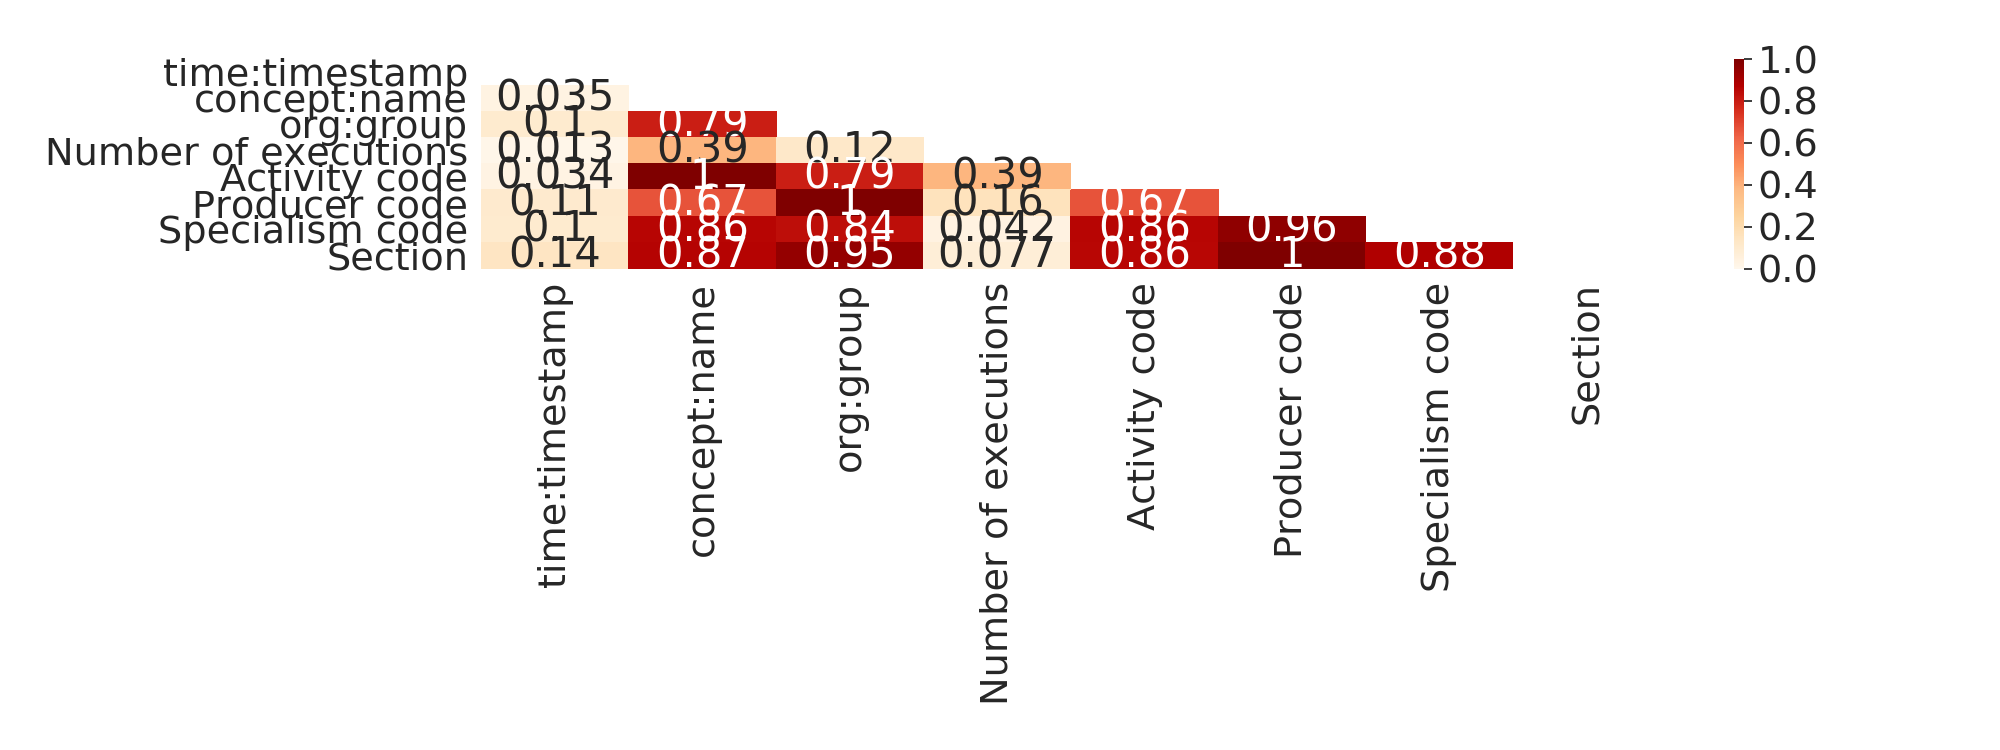
\includegraphics[width=\textwidth]{gfx/bpic2011/correlation-heatmap.png}
\caption{Heatmap of correlating values within the BPIC11 dataset, obtained using pair-wise application of Cramér's~V}
\label{fig:BPIC11-correlation-heatmap}
\end{figure}

\begin{figure}[ht!]
\centering
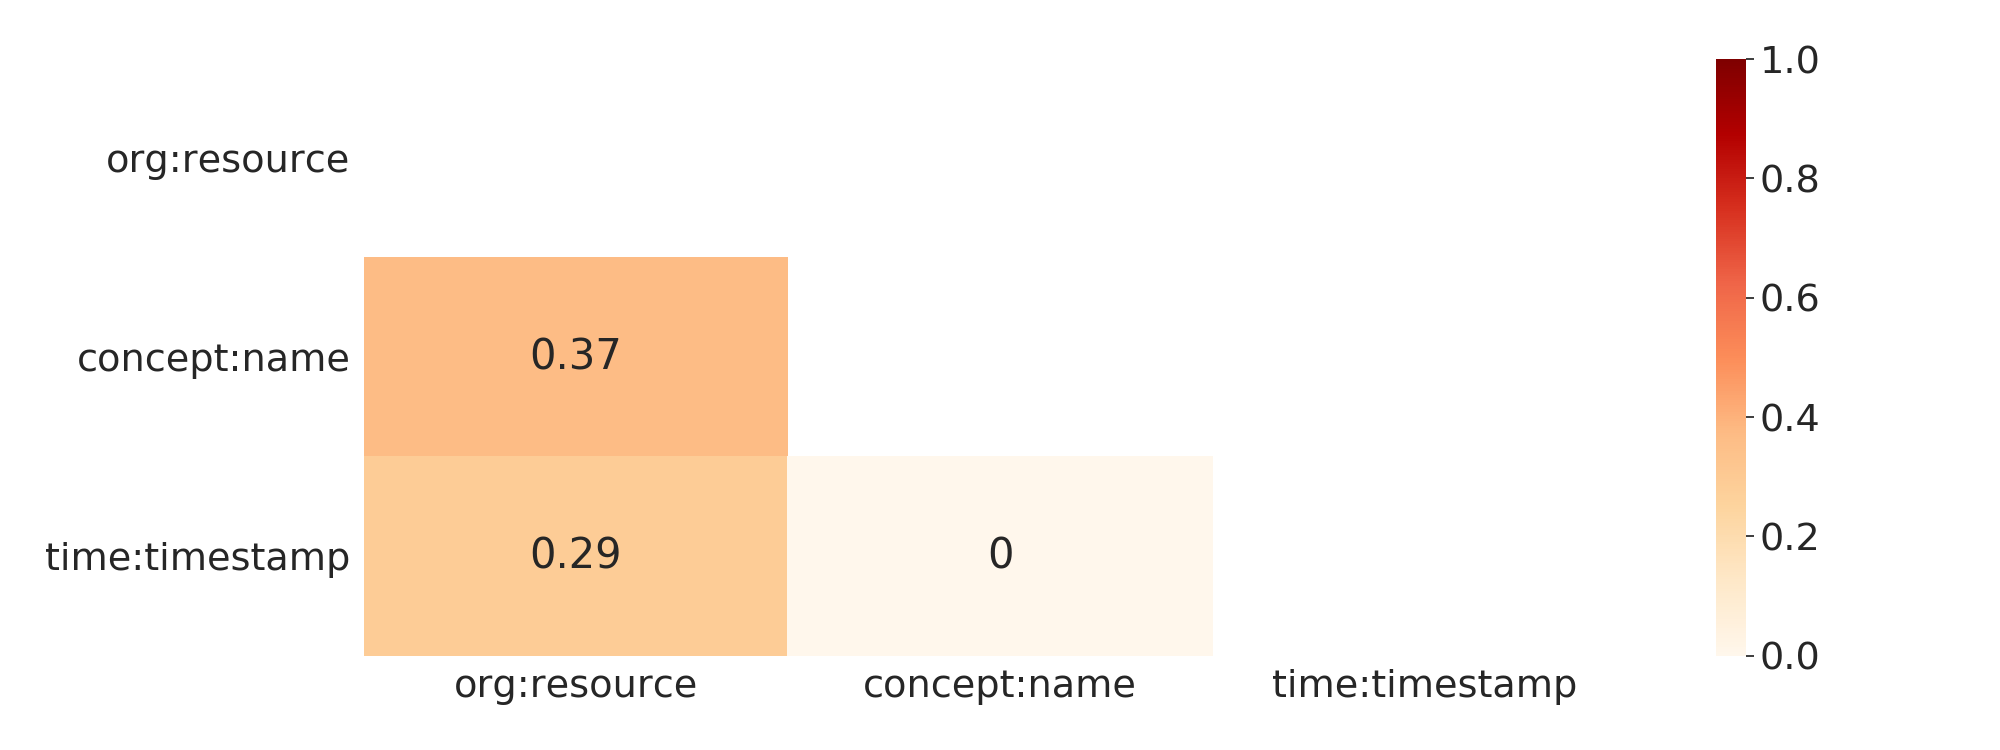
\includegraphics[width=\textwidth]{gfx/bpic2012/correlation-heatmap.png}
\caption{Heatmap of correlating values within the BPIC12 dataset, obtained using pair-wise application of Cramér's~V}
\label{fig:BPIC12-correlation-heatmap}
\end{figure}

\begin{figure}[ht!]
\centering
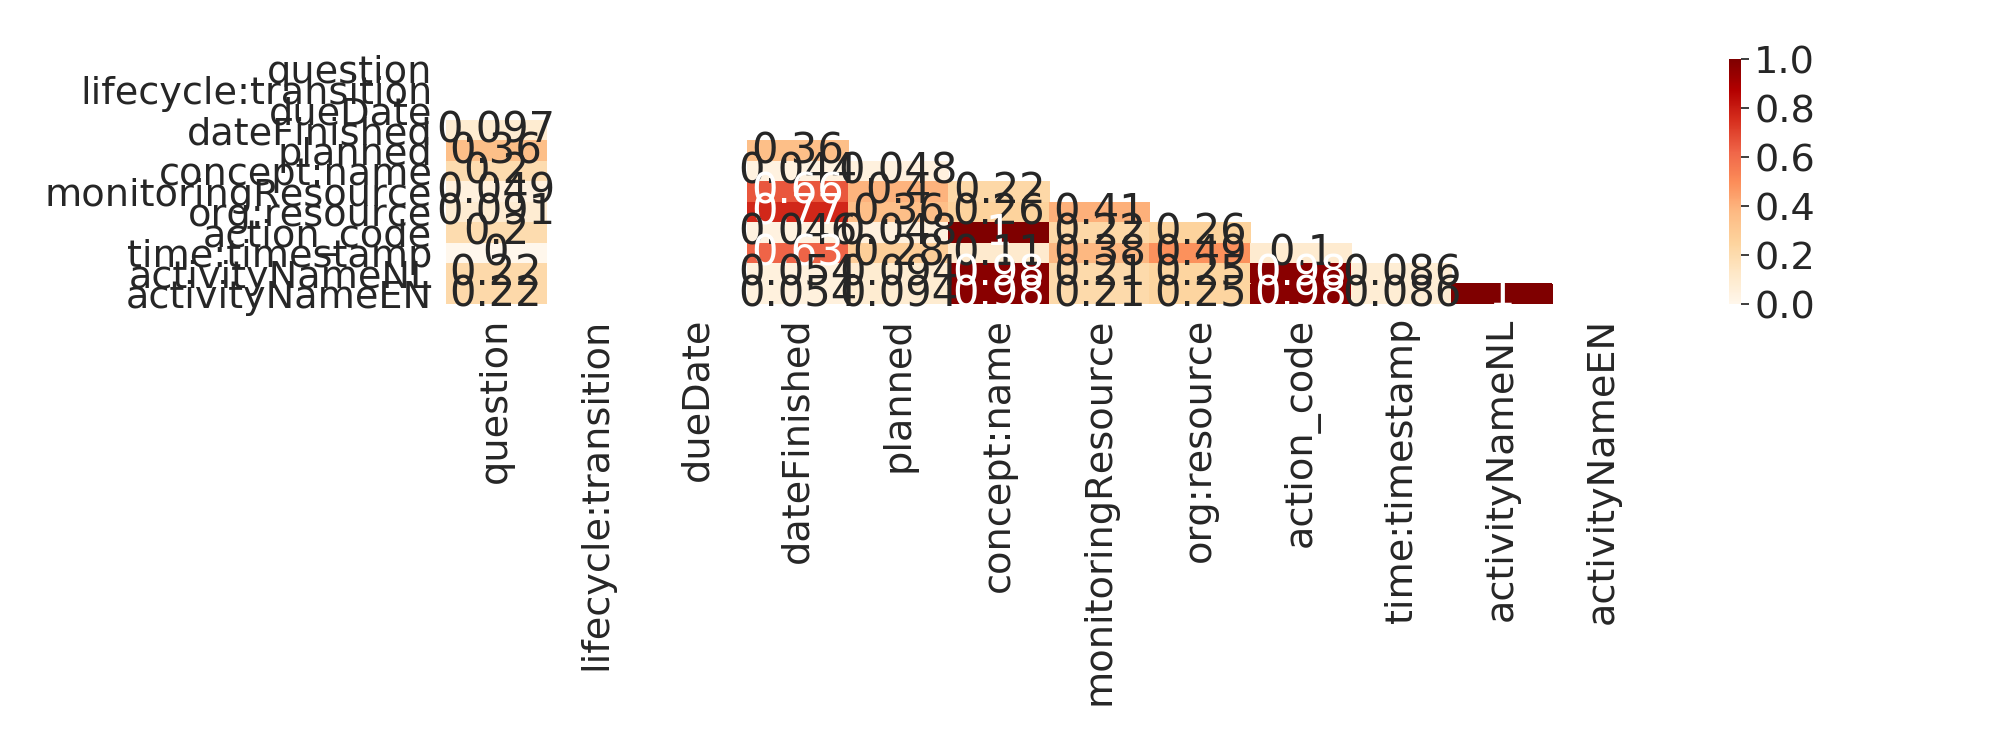
\includegraphics[width=\textwidth]{gfx/bpic2015_1/correlation-heatmap.png}
\caption{Heatmap of correlating values within the BPIC15-1 dataset, obtained using pair-wise application of Cramér's~V}
\label{fig:BPIC15-1-correlation-heatmap}
\end{figure}

\begin{figure}[ht!]
\centering
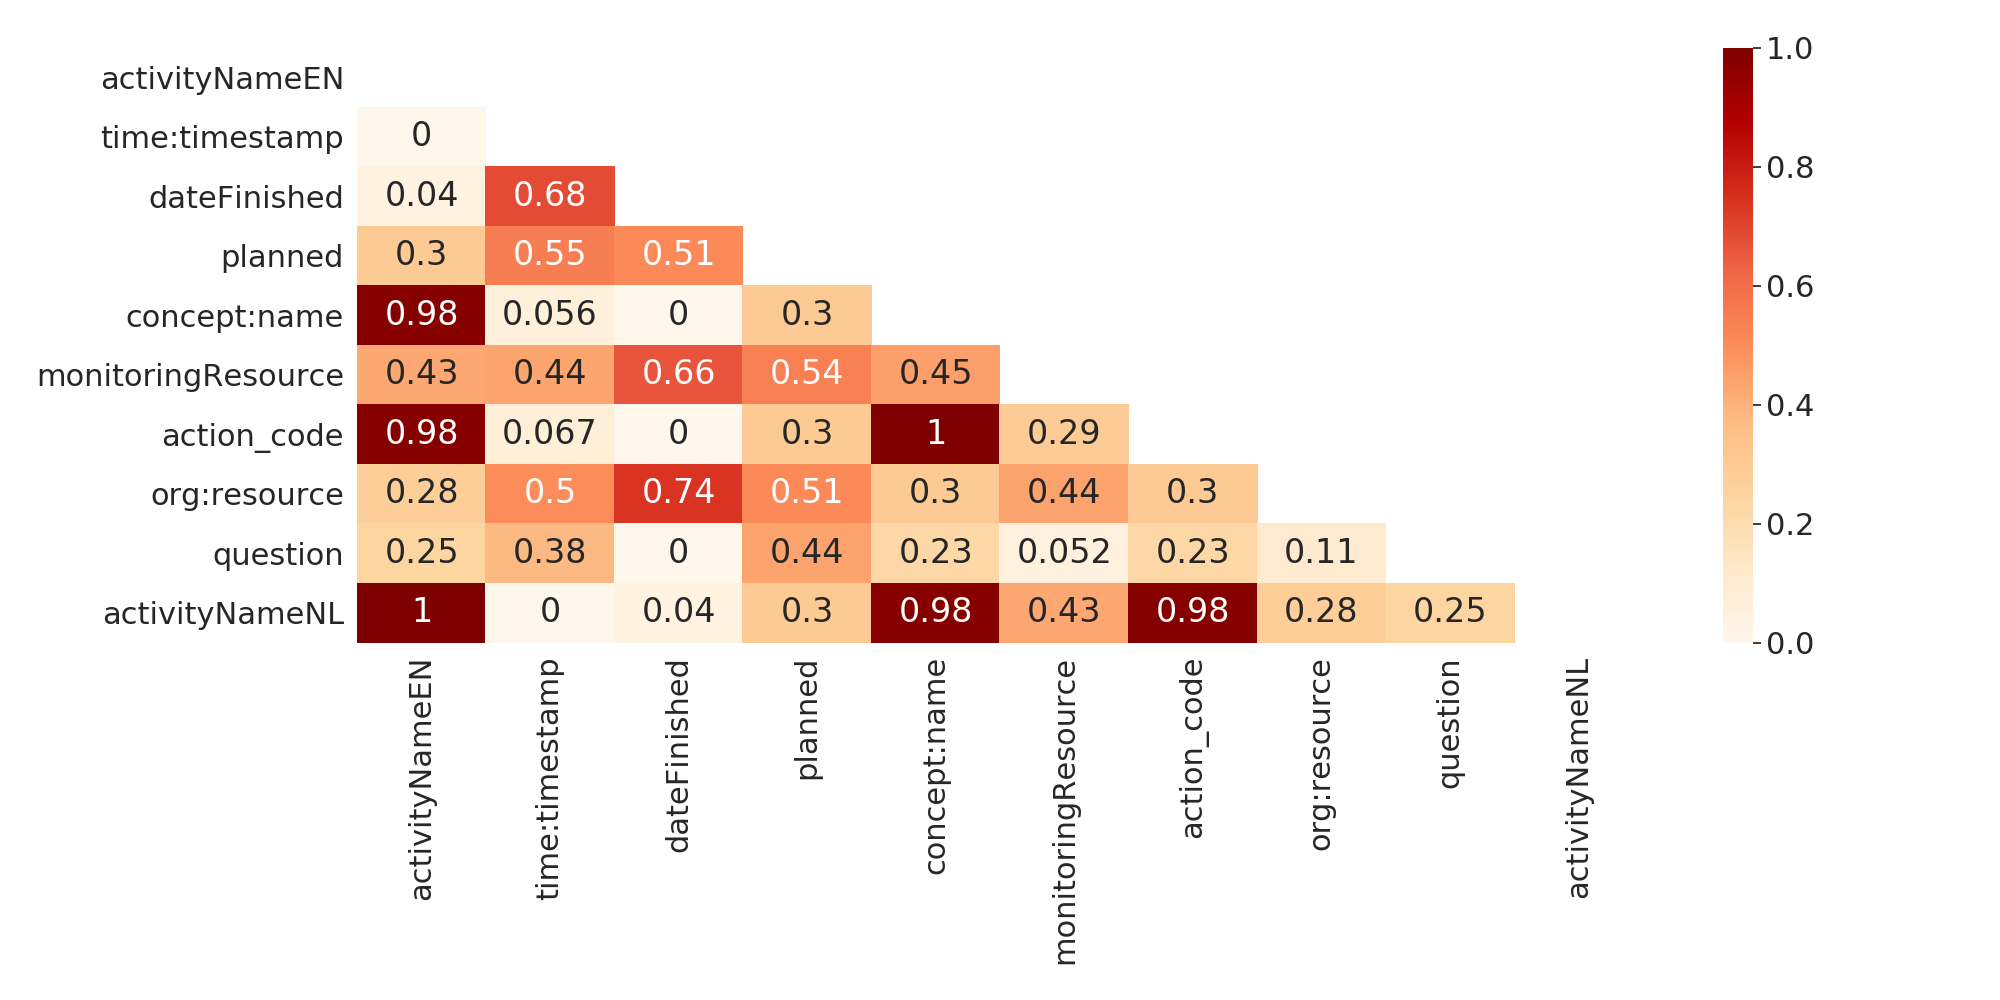
\includegraphics[width=\textwidth]{gfx/bpic2015_2/correlation-heatmap.png}
\caption{Heatmap of correlating values within the BPIC15-2 dataset, obtained using pair-wise application of Cramér's~V}
\label{fig:BPIC15-2-correlation-heatmap}
\end{figure}

\begin{figure}[ht!]
\centering
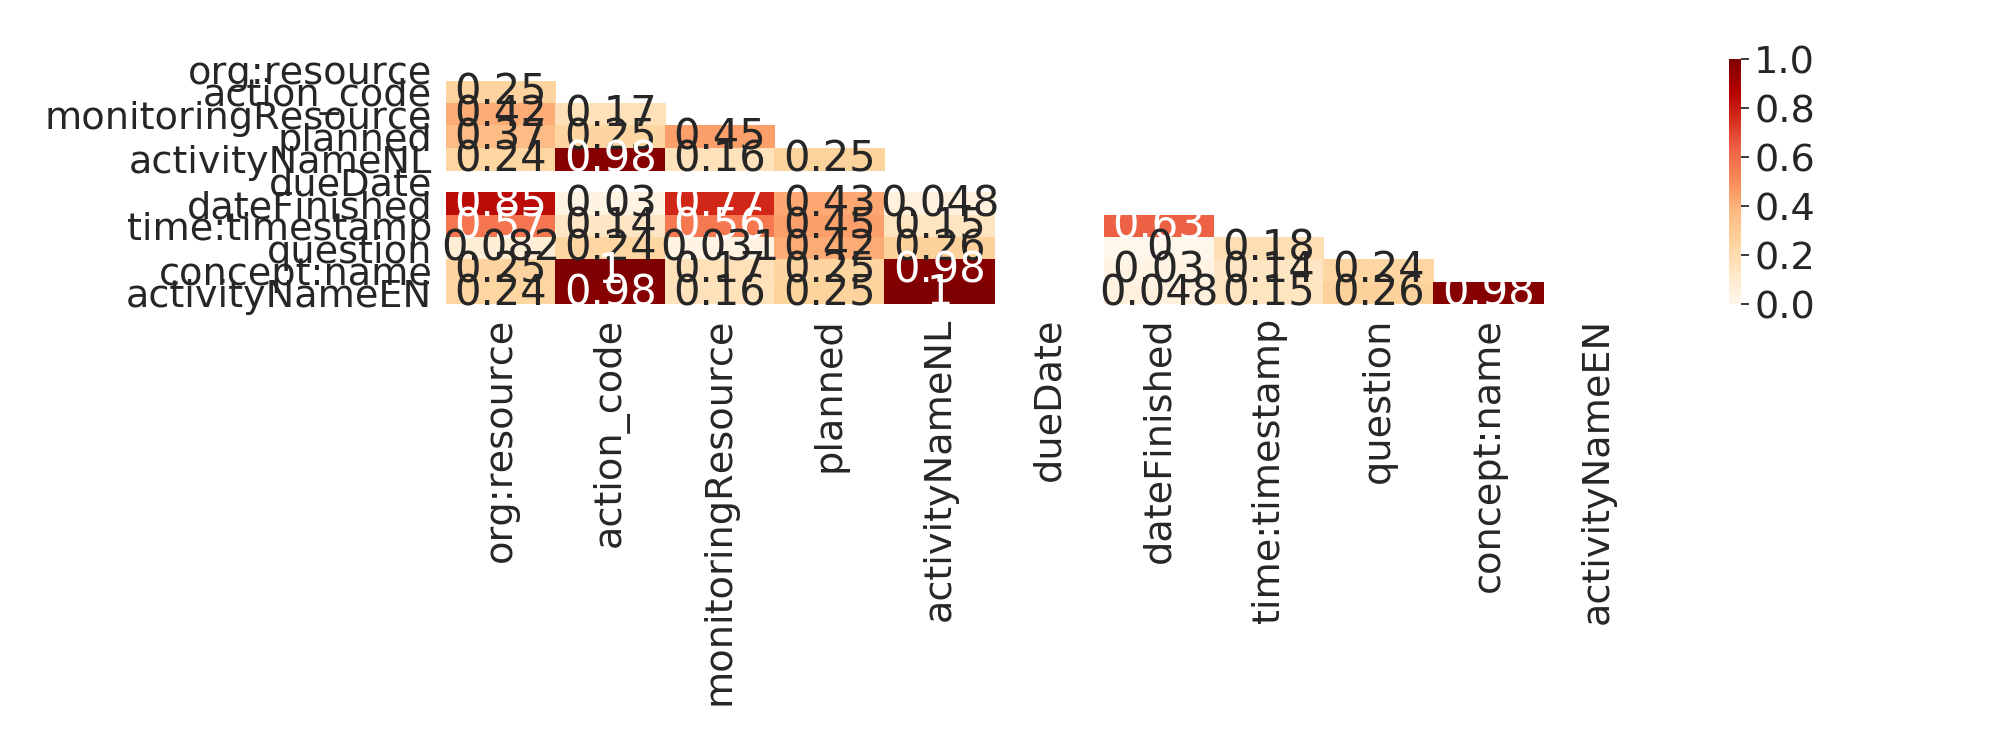
\includegraphics[width=\textwidth]{gfx/bpic2015_3/correlation-heatmap.png}
\caption{Heatmap of correlating values within the BPIC15-3 dataset, obtained using pair-wise application of Cramér's~V}
\label{fig:BPIC15-3-correlation-heatmap}
\end{figure}

\begin{figure}[ht!]
\centering
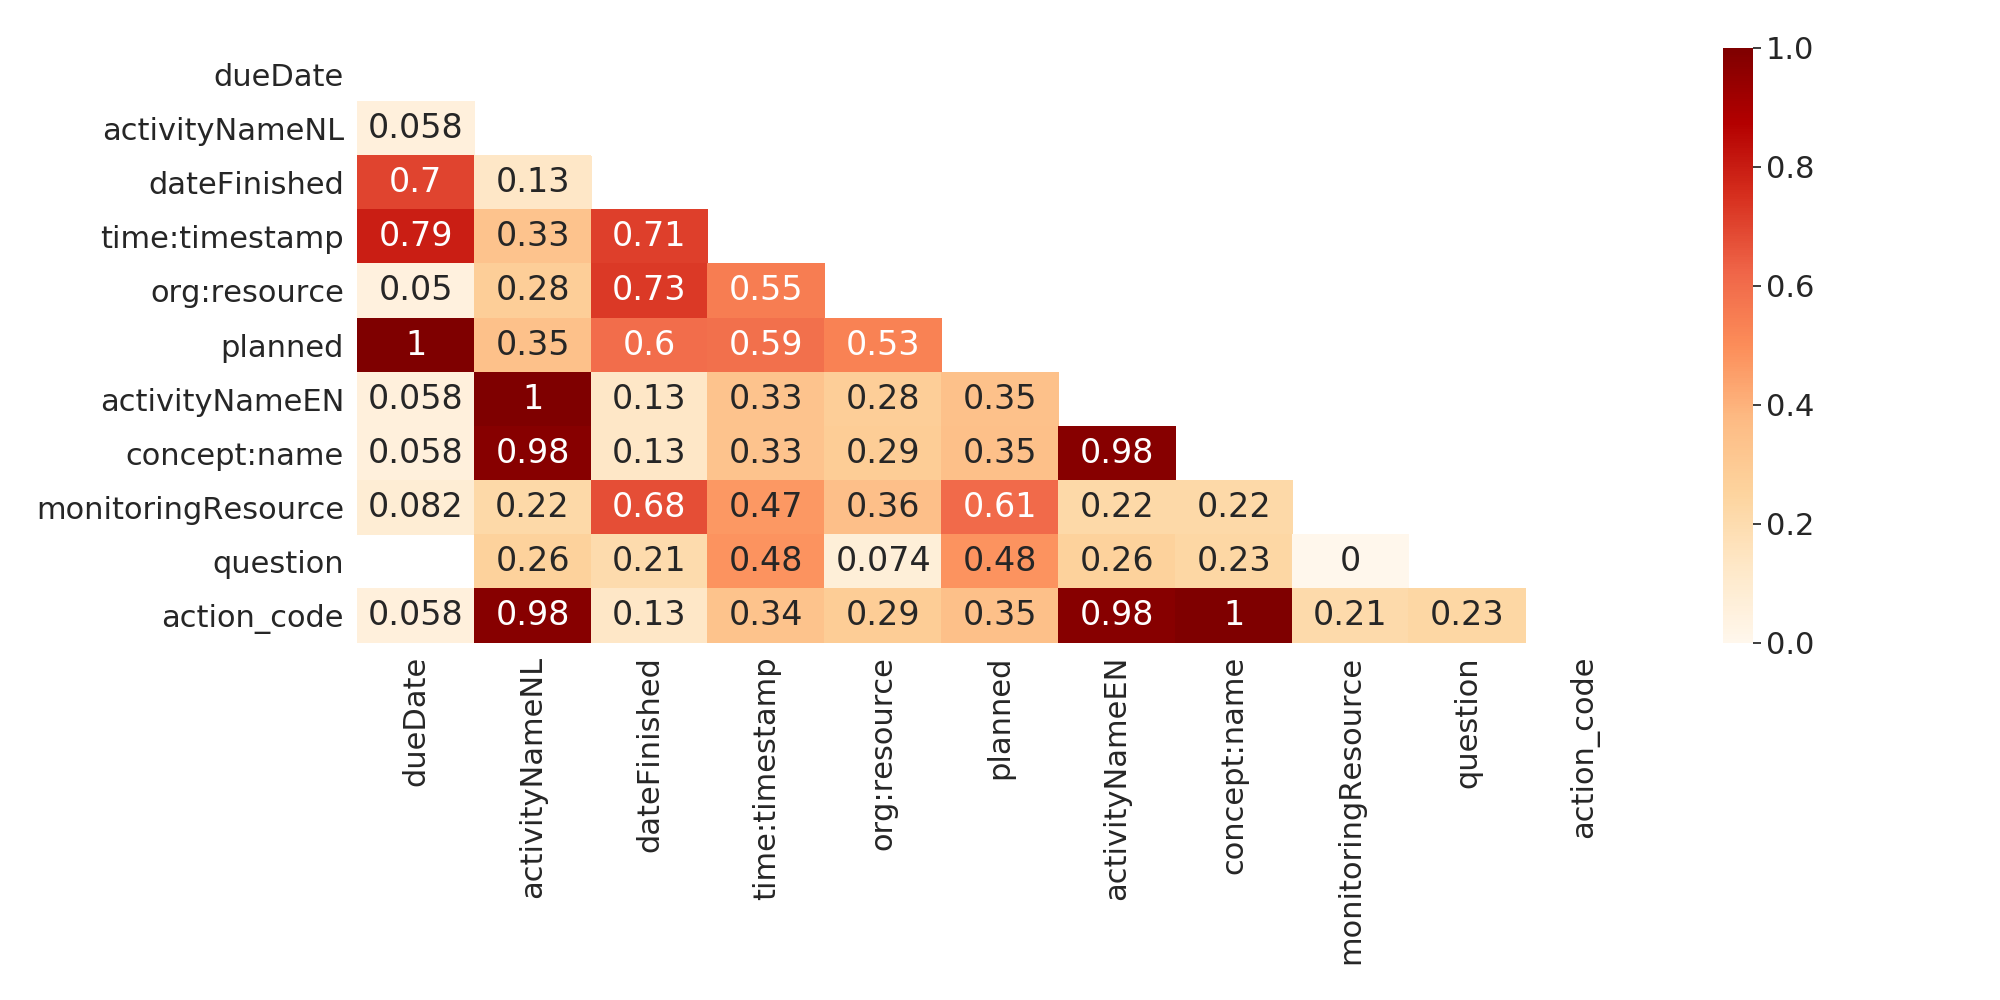
\includegraphics[width=\textwidth]{gfx/bpic2015_4/correlation-heatmap.png}
\caption{Heatmap of correlating values within the BPIC15-4 dataset, obtained using pair-wise application of Cramér's~V}
\label{fig:BPIC15-4-correlation-heatmap}
\end{figure}

\begin{figure}[ht!]
\centering
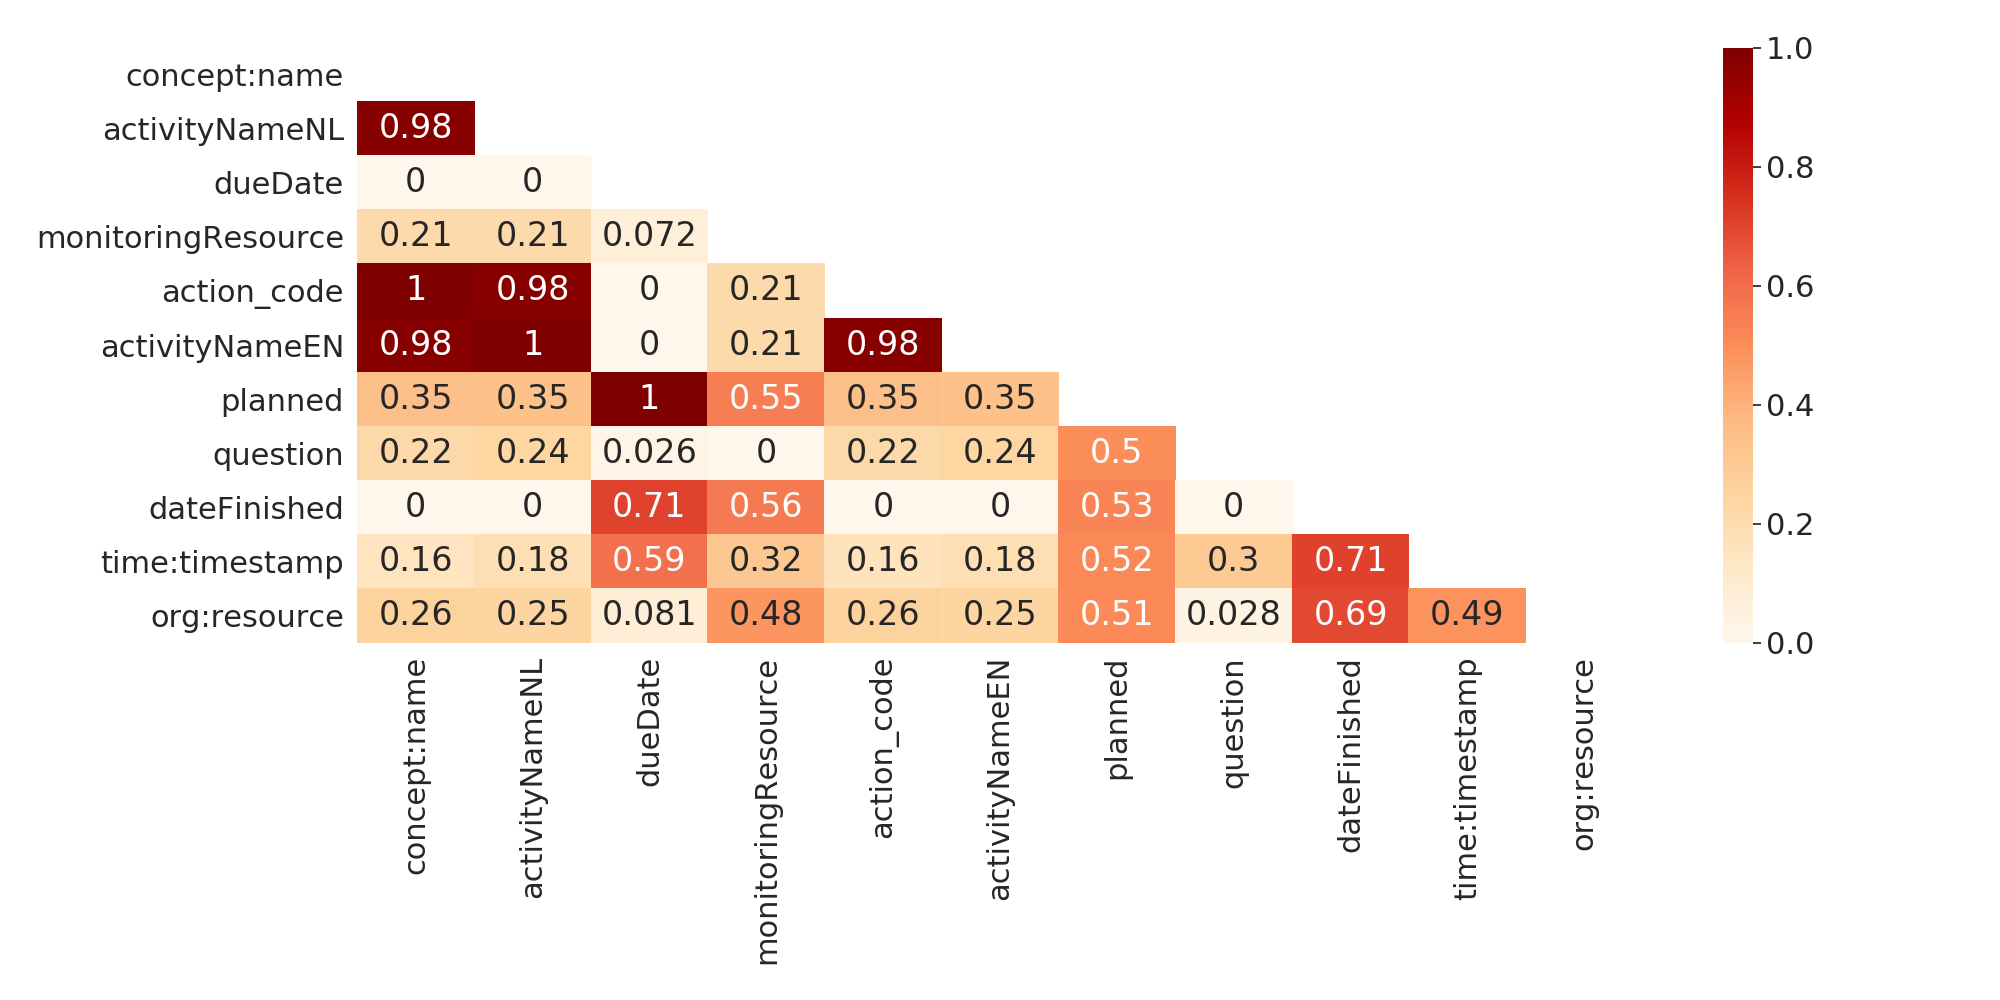
\includegraphics[width=\textwidth]{gfx/bpic2015_5/correlation-heatmap.png}
\caption{Heatmap of correlating values within the BPIC15-5 dataset, obtained using pair-wise application of Cramér's~V}
\label{fig:BPIC15-5-correlation-heatmap}
\end{figure}
